%%%%%%%%%%%%%%%%%%%%%%%%%%%%%%%%%%%%%%%%%%%%%%
% Head matter - can we try to be consistent on
% included packages
\documentclass{beamer}
\mode<presentation>
\usetheme{Copenhagen}
\usepackage[english]{babel}
\usepackage[utf8x]{inputenc}
\usepackage{graphicx}
\setbeamerfont{footnote}{size=\tiny}
\usepackage[style=authoryear,maxnames=1]{biblatex}
\addbibresource{mybib.bib} 
%%%%%%%%%%%%%%%%%%%%%%%%%%%%%%%%%%%%%%%%%%%%%%
% Formatting for title page
\title[]{Text Generation and Neural Style Transfer}
\author{S. Singhal, K. Siddarth, P. Agarwal, A. Garg \\ Mentor: N. Asnani}
\institute{Department of Computer Science and Engineering\\ IIT Kanpur}
\date{$22^{nd}$ November 2017}
%%%%%%%%%%%%%%%%%%%%%%%%%%%%%%%%%%%%%%%%%%%%%%
\AtBeginSubsection[]
{
  \begin{frame}<beamer>{Outline}
    \tableofcontents[currentsection,currentsubsection]
  \end{frame}
}

\begin{document}
\begin{frame}
  \titlepage
\end{frame}

%\section{Introduction}
% There is actually no point to the sections 
% since we are not using table of contents mark up

\begin{frame}{Introduction}
\begin{itemize}
  \item Text generation is a foundational task in Natural Language Processing
  \item The aim is to produce a natural language text in order to meet specified communicative goals.
  \item Takes non-linguistic representation of information as input and outputs text, documents, reports, etc.
  \item Has a diverse set of applications ranging from image captioning to text summarization.
\end{itemize}
\end{frame}
\begin{frame}{Goals}
	\begin{itemize}
	\item Attempt to generate coherent text in the style of an author
    \item Experiment with different models to see which works best
    \item Design a model that takes text in the style of one author and convert it to that of another author 
	\end{itemize}
\end{frame}

\begin{frame}{Previous work}
\begin{itemize}
\item Our work is inspired by Andrej Karpathy's use of character level RNN's to generate text
\item At every time-step it feeds in a character, and the RNN predicts the next character.
\end{itemize}
\end{frame}

\begin{frame}{Previous work}
\begin{figure}
        \includegraphics[width=0.8\linewidth]{1.pdf}
    \end{figure}
    \begin{itemize}
        \item $w_i$ - input tokens of source article       
        \item $h_i$ - Encoder hidden states
        \item $P_{vocab} = softmax(Vh_i + b)$ is the distribution over vocabulary from which we sample $out_i$
    \end{itemize}
\end{frame}

\begin{frame}{Previous work}
\begin{itemize}
\item Our work is inspired by Andrej Karpathy's use of character level RNN's to generate text
\item At every time-step we feed in a character, and the RNN predicts the next character.
\item One very basic problem with this model is that character RNN's can conjure up words on their own.
\item A very easy fix is to use word level models instead of character level models.
\end{itemize}
\end{frame}


\begin{frame}{Character vs Word}
\begin{itemize}
\item Both have size 512 and 3 stacked layers
\item Character level
\begin{block}{}
% 	  ome filler text??
%       konsa filler text?
% abhi
	\textbf{KINGequeses}, wifely
A mighty \textbf{vanagy} died, and is it \textbf{sotis} being note but by flatter, which,
I rather be! Hear over-blown swifled by;
The king was timely followed.
\end{block}
\item Word level
\begin{block}{}
King VI: First Citizen: And will will tell you, I have not I is to be content; it are not that is a more than all the writing. DUKE OF YORK: My lord, I am a bond, and we is the writing. DUKE OF YORK: What is the writing.
\end{block}
\end{itemize}
\end{frame}

\begin{frame}{2 vs 3 layers}
\begin{itemize}
    \item While testing, we found that having more layers with a vanilla RNN leads to nonsensical outputs
\end{itemize}
\begin{block}{2 layers}
KING RICHARD III: Ay, if you know the general is not so far with me. QUEEN ELIZABETH: My lord, I will not not a man of such good Than not to see him in the Duke of York. KING RICHARD III: Ay, but you will not be a traitor to the people, And yet thou art a soldier, and that is not so much with me for his eye
\end{block}

\begin{block}{3 layers}
KING of of of of of of of of of of of of of of of of of of of of of of of of of of of of of of of of of of of of of of of of of of of of of of of of of of of of of of of of of of of of of of of of of of of of of of of of of of of of of of of of of of of of of of of of of of of of
\end{block}
\end{frame}

\begin{frame}{RNN vs LSTM}
\begin{itemize}
\item Both have size of 1024 and 3 stacked layers
\end{itemize}
\begin{block}{RNN}
KING of of of of of of of of of of of of of of of of of of of of of of of of of of of of of of of of of of of of of of of of of of of of of of of of of of of of of of of of of of of of of of of of of of of of of of of of of of of of of of of of of of of of of of of of of of of of
\end{block}

\begin{block}{LSTM}
King VI: First Citizen: And will will tell you, I have not I is to be content; it are not that is a more than all the writing. DUKE OF YORK: My lord, I am a bond, and we is the writing. DUKE OF YORK: What is the writing. DUKE OF YORK: What is the writing.
\end{block}
\end{frame}




\begin{frame}{Sequence to Sequence models}

\begin{figure}
        \includegraphics[width=1.0\linewidth]{seq2seq2.png}
        % \caption{lion!!}
    \end{figure}
    \footnote{Image from colah.github.io}
\begin{itemize}
    \item It consists of an Encoder(Bidirectional LSTM) and a Decoder LSTM network.
    \item The final hidden state from the Encoder(thought vector) is passed into the Decoder.
\end{itemize}
\end{frame}

\begin{frame}{Attention}
	\begin{itemize}   
        \item $importance_{i,t} = V* tanh(e_iW_1+h_tW_2+b_{attn})$.
        \item Attention Distribution $a^t = softmax(importance_{i,t})$
        \item  Context vector $ h^{*}_t = \sum_i e_i*a^t_i$
    \end{itemize}
    \begin{figure}
            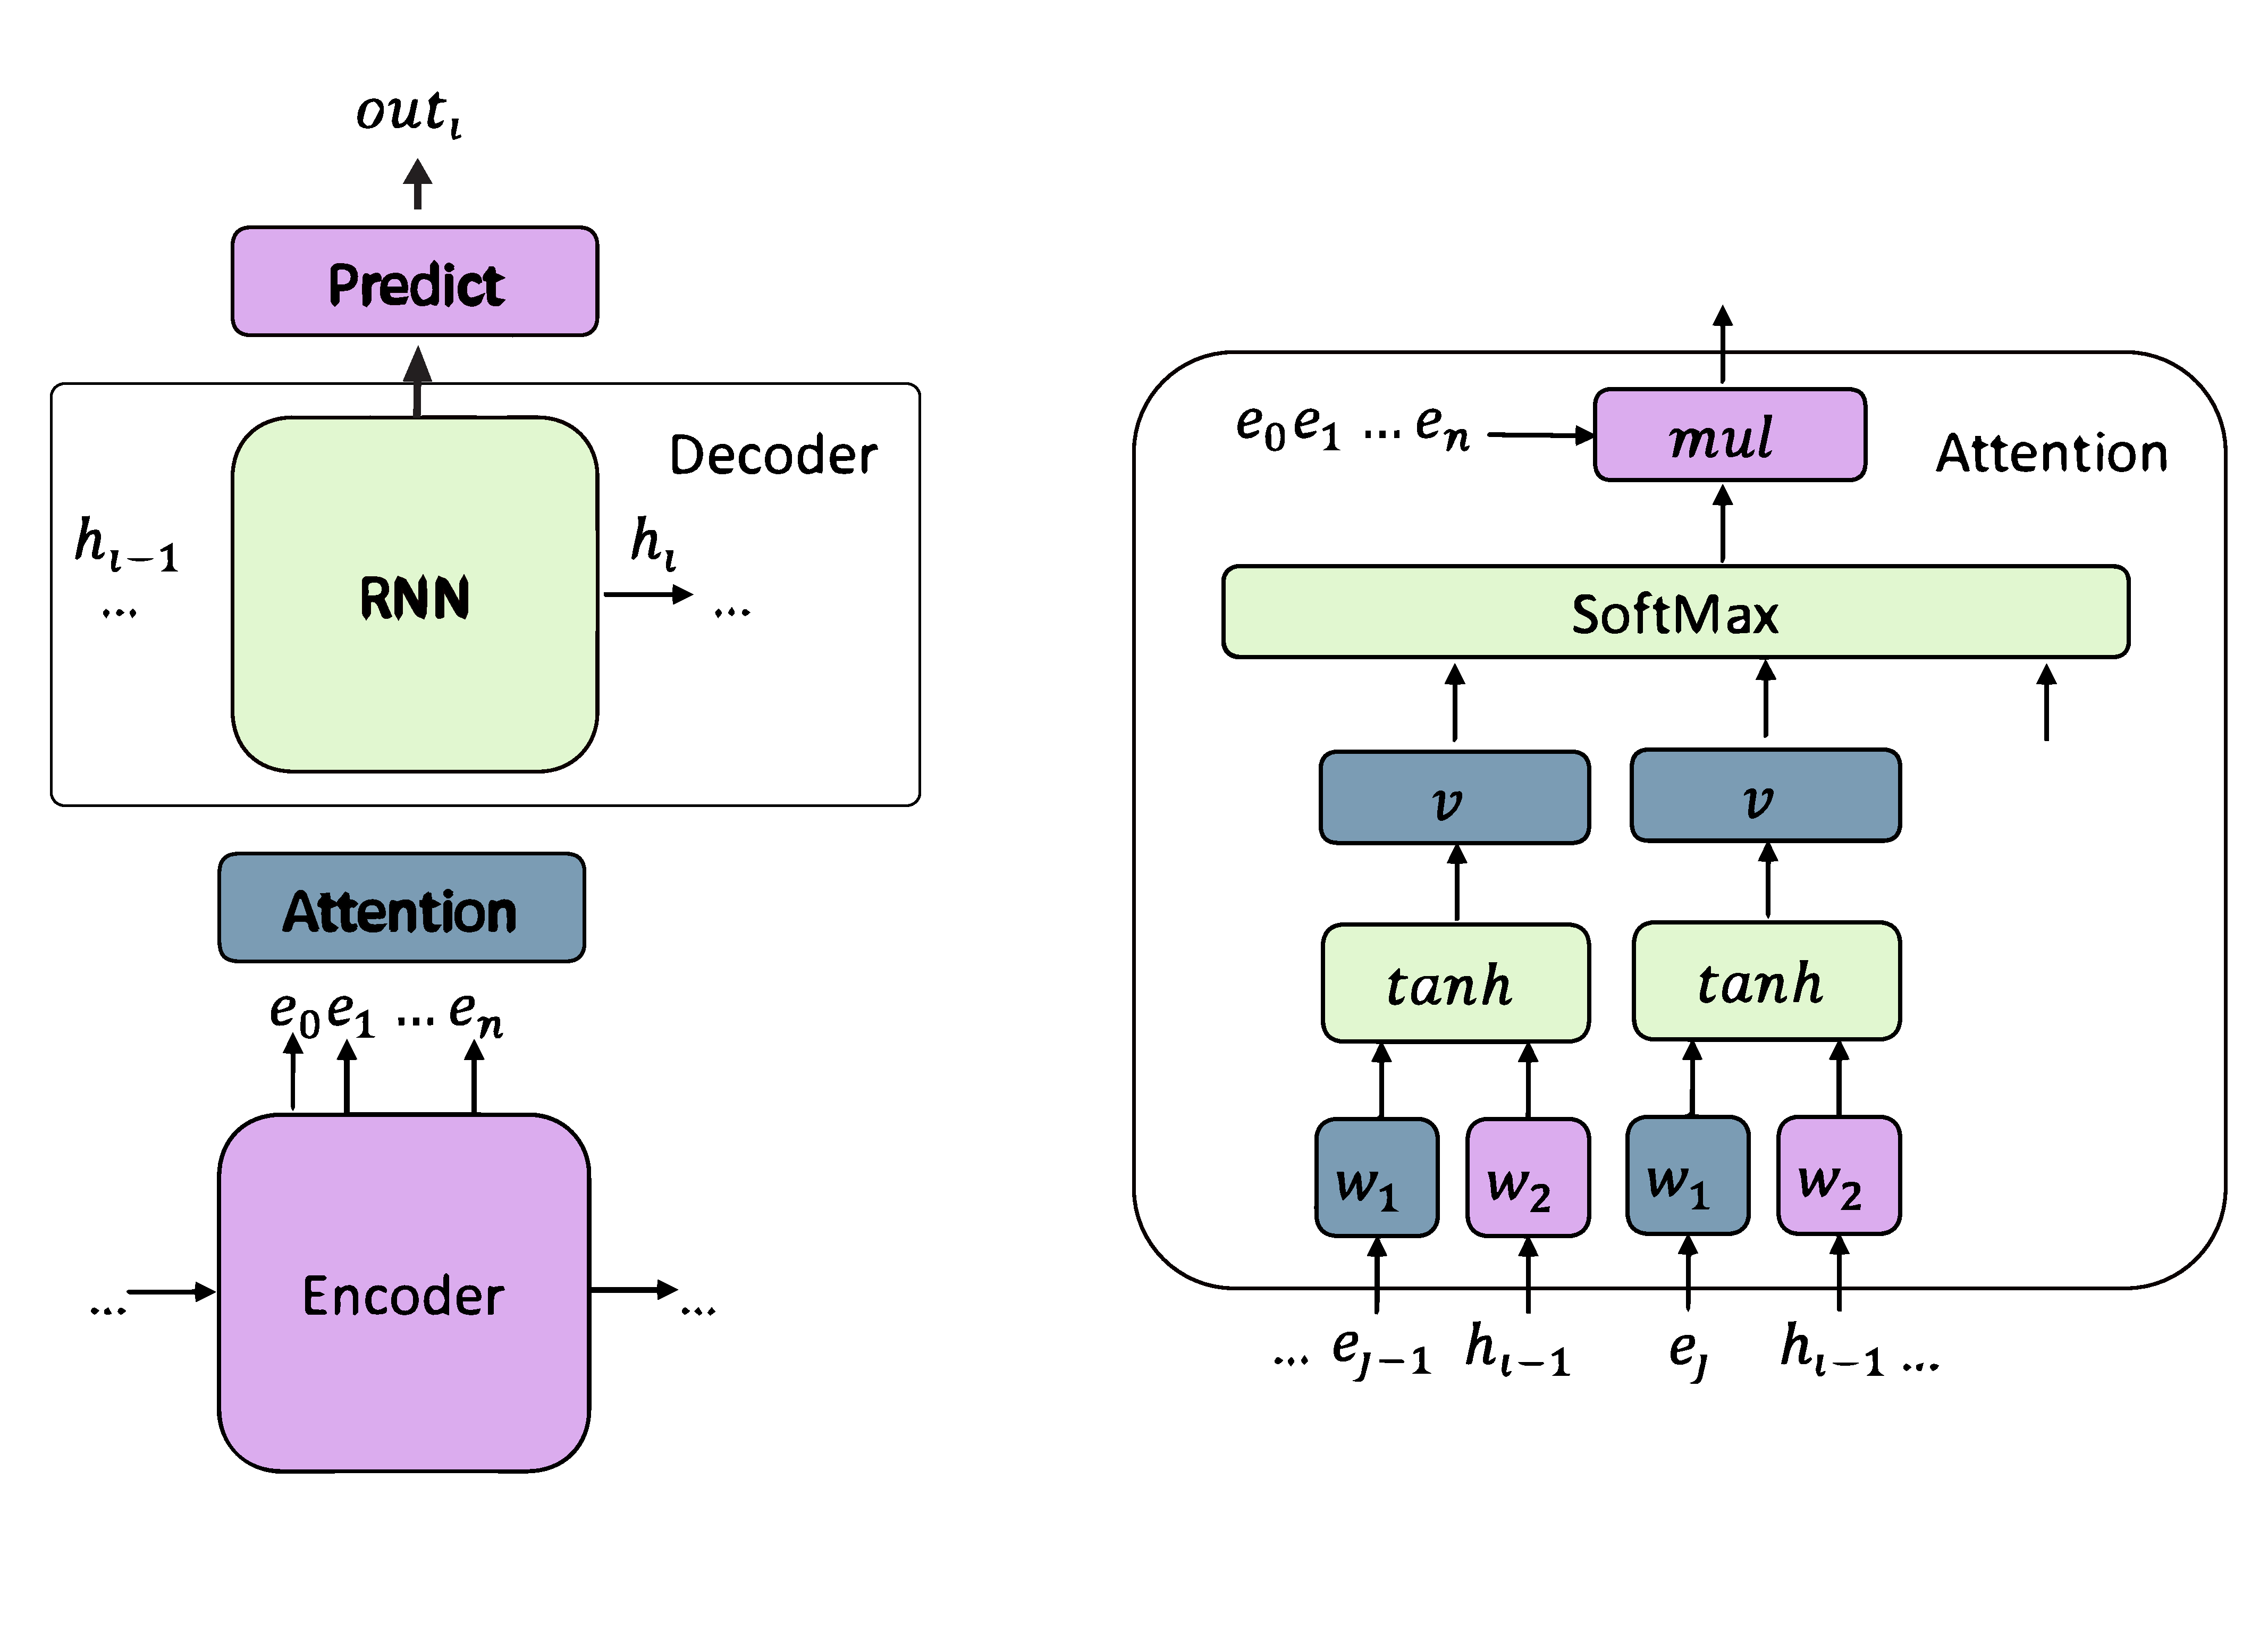
\includegraphics[width=0.7\linewidth]{7.pdf}
        % \caption{lion!!}
    \end{figure}
\end{frame}

\begin{frame}{Our Novel model}
	\begin{itemize}
	\item Inspired by the work of \cite{} in vision.
	\item They manage to separate the style of the image and the content of the image by passing the image through a CNN, and then reconstructing the image from the representation.
	\item This works in a very similar way to an autoencoder model.
	\end{itemize}
\end{frame}
\section{Style Transfer}
\begin{frame}{Style Transfer}
\begin{itemize}
\item Here we aim to take a corpus of text from one author and generate text with the same meaning in the style of another author.
\item There has not been much work on transfer of style from one author to another.
\item In the paper by Gatys et. al. [GEB15] he  authors  find  that  content  and  style  in  a  Convolutional  Neural  Net(CNN)  are  separable,  and therefore can be manipulated separately.
\end{itemize}
\end{frame}
\section{Our Novel Model}
\begin{frame}{Our Novel model}
We propose a very simple seq2seq model for style transfer.
\begin{block}{Step 1}
\begin{itemize}
    \item We make a seq2seq encoder-decoder work as an auto-encoder first. That is given an input sentence, we train it output the same sentence.
    \item We train this for \textbf{Author 1}. We did this for \texttt{Agatha Christie} and \texttt{Shakespeare}
    \item As these models can't handle multiple sentences well, we only train these on single sentence to single sentence
\end{itemize}
\end{block}
\begin{block}{Step 2}
\begin{itemize}
    \item Once the seq2seq auto-encoder is trained, we input the sentence of \textbf{Author 2} , in our case \texttt{Sir Arthur Conan Doyle}.
\end{itemize}
\end{block}
\end{frame}
\begin{frame}{Why should it work?}
\begin{itemize}
    \item We think that while training on the first author, the network would first learn a good encoding of that sentence. And then using that encoding it needs to learn regenerate the sentence.
    \item So it makes sense for the model to encode only the content part of the sentence in the encoding because style is same for the author and that can be learned by the decoder.
    \item We use different weights for encoder and decoder.
    \item So when, we feed in the sentence of second author it's content gets encoded by the encoder.
    \item Then the decoder styles that content in the style of the first author
\end{itemize}
\end{frame}

\begin{frame}{Parameters}
\begin{itemize}
\item LSTM
\item Size = 1024
\item Depth = 2
\item Embedding size = 500
\item beam width = 5
\item max decode step = 300
\end{itemize}
\end{frame}
\begin{frame}{How good is our Auto-Encoder}
\begin{itemize}
    \item We use the \texttt{BLEU} metric to test how well our model does self encoding
    \item We got a \texttt{BLEU} score of $55.13$, meaning it does the autoencoding pretty well
\end{itemize}
\end{frame}

\begin{frame}{Results}
    \begin{block}{Sherlock Holmes (Original)}
        Was there a secret marriage ? 
Absolutely none . 
None . 
No sign of it ? 
Come in ! \&; said Holmes .
Seven ! \&; I answered .
She will not sell . 
And I. 
My own seal . 
We have tried and failed . 
Stolen , then . 
I was mad - insane . 
To ruin me . 
We were both in the photograph . 
    \end{block}
    
    \begin{block}{Generated}
    Absolutely .
    None .
    ; No sign of it ? 
    Come in ! \&; said . 
    Lord ! &; I answered .
    She will not see . 
    And 
    My mother . 
    We have come and rushed . 
    Welcome , then . 
    I was mad - . 
    To me me . 
    We both were in the photograph .
    \end{block}
\end{frame}

\begin{frame}
\begin{block}{Original}
    How many ? I don't know . 
Holmes laughed .  It is quite a pretty little problem ,  said he .
 My photograph . 
 Stolen . 
What do you make of that ? asked Holmes .
 I am about to be married . 
 I think that I had better go , Holmes . 
 My private note-paper . 
 No legal papers or certificates ? 
 I promise ,  said Holmes .
I carefully examined the writing , and the paper upon which it was written .

\end{block}

\begin{block}{Generated}
 What do you make of that ?  asked asked .
 I am going to be married .
 I think that I had really go , I had
 My private private .
 No girl or or two ? 
 I dare , said gruffly .
I carefully the man , and the paper paper which it was written .
\end{block}
\end{frame}
\section{Ongoing Work}
\begin{frame}{Ongoing Work}
\begin{itemize}
    \item We plan to train two auto-encoder (A1-D1) and (A2-D2) for author 1 and 2 respectively.
    \item Then combine the A1 and D2 to get a style transfer model to convert text from author 1 to author 2.
    
    
\end{itemize}
    
\end{frame}

%\section{Some \LaTeX{} Examples}\
%\subsection{Tables and Figures}


\appendix
\section<presentation>*{\appendixname}
\subsection<presentation>*{References}

\begin{frame}[allowframebreaks]
  \frametitle<presentation>{References}
    
  \begin{thebibliography}{10}
    
%   \beamertemplatebookbibitems
  % Start with overview books.

  \beamertemplatearticlebibitems
  
  \bibitem{Author1990}
    A. Karpathy
    \newblock { The Unreasonable Effectiveness of Recurrent Neural Networks}.
    \newblock {\em Andrej Karpathy blog} 2015.
 
    
  % Followed by interesting articles. Keep the list short. 

  \bibitem{Someone2000}
    Bahdanau, Dzmitry and Cho, Kyunghyun and Bengio, Yoshua
    \newblock Neural machine translation by jointly learning to align and translate.
    \newblock {\em arXiv preprint arXiv:1409.0473}, 2014.
    
  \bibitem{asdf}
    Leon A. Gatys, Alexander S. Ecker, Matthias Bethge
    \newblock A Neural Algorithm of Artistic Style
    \newblock{\em arXiv preprint} arXiv:1508.06576, 2015
    
      \bibitem{aswdf}
   Zhiting Hu, Zichao Yang, Xiaodan Liang, Ruslan Salakhutdinov, Eric P. Xing
    \newblock Toward Controlled Generation of Text
    \newblock{\em arXiv preprint}  	arXiv:1703.00955, 2017
  \end{thebibliography}


 \printbibliography
\end{frame}


% \bibliographystyle{plain}
% \bibliography{references}
\end{document}
